\documentclass{unswmaths}
\usepackage{unswshortcuts}
\usepackage{dsfont}
\usepackage[hyphens]{url}
\begin{document}
\author{Adam J. Gray}
\title{Assignment 2}
\subject{Complex Analysis}
\studentno{3329798}

\newcommand{\llra}{\Leftrightarrow}

\unswtitle

\section{}

\begin{center}
	Yes.
\end{center}

We'll answer this question in steps.

Firstly we cite Carath{\'e}odory's theorem.

\begin{theorem}[Carath{\'e}odory's Theorem]
Suppose $ U $ is a simply connected open subset of $ \Cplx $, whose boundary is a Jordan curve $ \gamma $ then the Riemann map
\begin{align}
	f:U\lra D
\end{align}
from $ U $ to the unit disk $ D $ extends \emph{continuously} to the boundary.
\end{theorem}
Note that  by \emph{Jordan curve} we mean a curce which is non-self-intersecting and forms a continuous loop in $ \Cplx $. 

Carath{\'e}odory's theorem is not sufficient to solve the problem however, as it does not guarantee analyticity for this we are going to need the Schwarz reflection principle. 

By using the appropriate change of variables we can map any of the straight sides to the triangle to the real line and then apply the principle.
Instead of considering the conformal mapping form the circle to the triangle, we consider the conformal mapping from the upper half plane to the triangle. (Note that we can do this because we can conformally map the unit ball to the upper half plane and then apply this result.

The basic idea is to consider the map $ f : U \lra D $. Since $ z \in \partial U $ means that $ f(z) \in \partial D $ we can say that $ \lambda(z) = \log|f(z)| $ is real valued, but further that on $ U $ $ z \lra \partial U $ means that $ \lambda(z) \lra 0 $, except at perhaps $f^{-1}(0) $. The Schwarz reflection principle can therefore be applied to  $ \lambda $ to give an analytic extension of $ \lambda $ in some neighbourhood of $ \partial U $. Locallhy $ \lambda $ is real but it can be viewed as the real part of some holomorphic function, say $ h $. We choose the imaginary part such that $ e^h \equiv f $ in $ U $. This then gives us the analytic extension we have been looking for. We call this new function $ \tilde{g} $.  If we take the domains of the reflected extensions small enough then it will be possible to say that this new open set $ \tilde{U} $ that $ \tilde{g} $ is defined on is conformally equivalent to some open set containing $ D $. 
\newline

A further explanation of how this works can be found in L. Ahlfors Complex Analysis. McGraw-Hill New York 1979.  

A good explanation of the Schwarz reflection principle can be found in Axler, Bourdon and Ramey's Harmonic Function Theory, Springer, 2000.

The idea for how to get this to work came from \url{http://math.stackexchange.com/questions/752676/analytic-continuation-of-a-conformal-map}.


\section{}
We recall Runge's theorem.
\begin{theorem}
Let $K $ be a compact subset of $ \Cplx $ and let $ f $ be a function which is holomorphic on an open subset containing $ K $. If $ A $ is a set containing at least one complex number from every bounded component of $ \Cplx \setminus K $ then there exists a sequence $ \left\{ r_n\right\}_{n \in \mathbb{Z}} $ of rational functions which converges uniformly to $ f $ on K and such that all the poles of the functions $ \left\{ r_n\right\}_{n \in \mathbb{Z}} $ are in $ A $.  
\end{theorem}

An important corollary of Runge's theorem is the following
\begin{corollary}
	If $ K $ is a compact subset of $ \Cplx $ such that $ \Cplx \setminus K $ is a connected set and $ f $ is a holomorphic function on $ K $, then there exists a sequence of polynomials which approaches $ f $ uniformly on $ K $.
\end{corollary}

This corollary is important as it will allow us to construct a sequence of polynomials whose limit is discontinuous. 

Consider the sequence of sets $ K_n $ and $ L_n $ as described in figure \ref{fig:1}. Importantly note that $ \Cplx \setminus L_n $ is connected. This means we can apply the corollary to Runge's theorem.
\begin{figure}[h]
	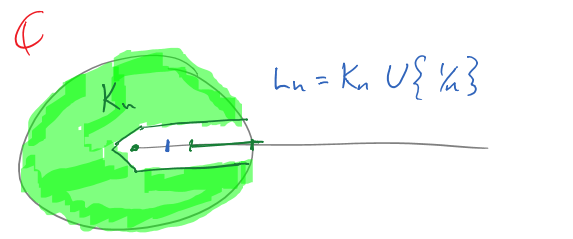
\includegraphics[scale=1]{ComplexDomainTask2Qn2}
	\caption{$K_n = \{ z \in \Cplx : |z| \leq 1, \operatorname{dist}(z, \Rl_+) \geq 1/n \} \cup [2 / n, 1] \cup \{0 \}$ and $ L_n = K_n \cup \{ 1 / n \} $}
		\label{fig:1}
\end{figure}

Let $ f_n $ be a holomorphic function on a (non-connected) neighbourhood of $ L_n $ such that $ f_n(z) = 0 $ for any $ z \in K_n $ but $ f_n(1/n) = 1 $. By Runge's theorem, there must exist a polynomial $ p_n $ such that $ |p_n - f_n| < 1/n $ on $ L_n $. Now we can see that $ p_n \lra 0 $ pointwise  on the unit disk. The convergence is not uniform however, as on some neighbourhood of $ 0 $ we have $ |p_n(1/n) - 1| \leq 1/n $.

Although we have constructed a counter example there is a remarkable theorem that almost guarantees the the limit function will be analytic. 

Osgood, Montel and Lavrentiev, \cite{Osgood1936} and Hartogs and Rosenthal\cite{Hartogs1928} go into this subject quite deeply. 

Osgood showed that if a sequence of polynomials converges pointwise in a region $ D $, then the limit function is analytic except for a closed nowhere dense set.

Note this solution is based of ideas from 

\url{http://mathoverflow.net/questions/117633/a-question-about-the-limit-of-a-sequence-of-pointwise-convergent-analytic-funtio} 

and

\url{http://math.stackexchange.com/questions/113240/pointwise-convergence-of-sequences-of-holomorphic-functions-to-holomorphic-funct}

\section{}

Let $ G_1 $ be the group of all conformal mappings from the unit ball into itself and let $ G_2 $ be the set of all conformal mappings from the upper half plane into itself. The group operation in both cases is function composition.  We claim that these two groups are isomorphic. 

Let $ D_1 = \{ z \in \Cplx : |z| < 1 \} $ and let $ U = \{ z : \Im(z) > 1 \} $.

Define the mapping $ M : D_1 \lra U $ by
$$ M(z) = \frac{(z+1)(1-i)}{2(z-i)}.$$
This is a Mobius transformation, so it is a conformal mapping and importantly bijective. 

We can produce an \emph{induced} transformation $ M_G : G_1 \lra G_2 $ where for $ f \in G_1 $
$$
	(M_G f)(x) = (M \circ f \circ M^{-1})(x).
$$
Obviously the inverse transformation $ M^{-1}_G : G_2 \lra G_1 $ is given by 
$$
	(M^{-1}_G f)(x) = (M^{-1} \circ f \circ M)(x) 
$$
for $ f \in G_2 $.

We just have to show that this is a group homomorphism.  

For $ f_1, f_2 $ in $ G_1 $
$$ M_G(f_1 \circ f_2) = M\circ f_1 \circ f_2 \circ M^{-1} = M\circ f_1 \circ M^{-1} \circ M \circ f_2 \circ M^{-1} = M_G(f_1) \circ M_G(f_2) $$
and so $ M_G $ is a group homomorphism. 

Thus the groups $ G_1 $ and $ G_2 $ are isomorphic. 

\section{}
Let $ D $ be a multiply connected domain. Let $ D_0 $ be its convex hull. Then pick an $ a \in \partial D $. Such an $ a $ must exist in $ D_0 $ as $ D $ is multiply connected.

Then the function $ f : D \lra \Cplx $, $$ f(z) = \frac{1}{z-a} $$ cannot be analytically extended to all of $ D_0 $. The reason being that no only an immediate continuation could be applied as it is in the boundary and clearly no immediate continuation would exist.


\section{}

We can identify any Mobius transformation 
\begin{align}
    f(z) = \frac{az + b}{cz + d} \sim \left[ \begin{array}{cc} a & b \\ c & d \end{array}\right]
\end{align}
with a matrix in $ GL_2(\mathbb{C}) $.

Also see that if
\begin{align}
    f \sim \left[ \begin{array}{cc} a & b \\ c & d \end{array}\right] \\
    g \sim \left[ \begin{array}{cc} e & f \\ g & h \end{array}\right] 
\end{align}
then
\begin{align}
    (g \circ f) &\sim \left[ \begin{array}{cc} e & f \\ g & h \end{array}\right] \left[ \begin{array}{cc} a & b \\ c & d \end{array} \right] \\
    &\sim \left[ \begin{array}{cc} ea + fc & eb + fd \\ ag + ch & gb + dh\end{array}\right].
\end{align}
Notice that this identification is not unique as
\begin{align}
    \frac{az + b}{cz+d} \sim \lambda\left[ \begin{array}{cc} a & b \\ c & d \end{array}\right]
\end{align}
for $ \lambda \in \Cplx $.

Either way we are interested in Mobius transformations which map the unit disk $ D_1 $ to itself. We claim that this consists of all the Mobius transformations of the form
\begin{align}
	f(z) = e^{i\theta} \frac{z+b}{\bar{b} z + 1 } \sim e^{i\theta} \left[ \begin{array}{cc} 1 & b \\ \bar{b} & 1\end{array} \right]
\end{align}
where $ \theta \in \Rl $ and $ b \in \Cplx $ with $ |b| < 1 $. 

This is possible to see from the three point construction of a Mobius transformation. This guarantees that the transformation specified by three points is unique. 

We now want to break this generic transformation up into its finite subgroups.

Suppose firstly that $ \theta = [0] $. Then the fixed points of the transformation are found by
\begin{align}
	z 	&= \frac{z + b}{\bar{b}z + 1} \\
	z(\bar{b}z + 1) &= z + b \\
	\bar{b}z^2 &= b \\
	z = \sqrt{\frac{b}{\bar{b}}}.
\end{align}

So the group of transformations generated (through repeated application) by
\begin{align}
	\frac{z+b}{\bar{b}{z} + 1}
\end{align}
has a global fixed point (actually 2) given by $ z = \sqrt{ b / \bar{b}} $.

If we allow $ \theta \neq [0] $ then the fixed points correspond to the solutions of the quadratic
\begin{align}
	z(\bar{z} + 1) = e^{i\theta}(z+ b).
\end{align}
We require the group to be finite. 
requiring that $ \theta \in 2\pi \mathbb{Q} $ and to
\begin{align}
	|z| = \left| \frac{z+b}{\bar{b}z + 1} \right|.
\end{align}
The reason for the first requirement is that otherwise rotations would never bring you back to the same point and so the group would be infinite. The reason for the second requirement is that if
\begin{align}
	|z| > \left| \frac{z+b}{\bar{b}z + 1} \right|.
\end{align}
then $ |f(e^{i\theta})| > 1 $. Also the inverse must be in the group so if 
\begin{align}
	|z| > \left| \frac{z+b}{\bar{b}z + 1} \right|.
\end{align}
then $ |f^{-1}(e^{i\theta})| > 1 $.
We therefore wish to find the conditions on $ b $ under which $ |f(z)| = |z| $. 

We only need to check
\begin{align}
	|\bar{b}z + 1| = |z + b|
\end{align}

but this last requirement means that $ b = 0 $ which just leaves us with transformations of the form
$ f(z) = e^{i \theta} z $ which are just rotations. So long as $ \theta \in 2\pi\mathbb{Q} $ the group generated by any number of rotations will be finite, with a single global fixed point of 0.

\begin{thebibliography}{9}

\bibitem{Osgood1936}
	Osgood, Montel and Lavrentiev,
	\emph{Sur les fonctions d'une variable complexe representable par des series de polynomes},
	Paris,
	1936
\bibitem{Hartogs1928}
	Hartogs and Rosenthal,
	\emph{Uber Folgen analytischer Funktionen},
	Math Ann.,
	1928,
	100,
	212-263
\end{thebibliography}

\end{document}
